\chapter{Context, Problems, and Related Works}\label{c2}%
This chapter reviews related works to contexts and problems. Give
chapter organization if necessary (or its too long)
%
\section{Whatever}\label{c2:s1} Whatever technique
you need here...

\begin{enumerate}[(a)]
\item Item 1
\item Item 2~\cite{j1}.
\end{enumerate}

\begin{equation}
y_i=\sum_{j=1}^Ni\frac{z^3}{y+z}
\end{equation}

\begin{subequations}
\label{c2:e1}
\begin{eqnarray}
\textbf{x} &=& \{x_1, x_2, \cdots, x_m\}
\\ &\approx&\{\textbf{x}_1, \textbf{x}_2,\cdots, \textbf{x}_n\}
\end{eqnarray}
\end{subequations}
%
Equation~(\ref{c2:e1}) represents whatever...

This is how you should call a figure, shown here as
Figure~\ref{c2:f1}

\begin{figure}[!ht]
    \centering{
    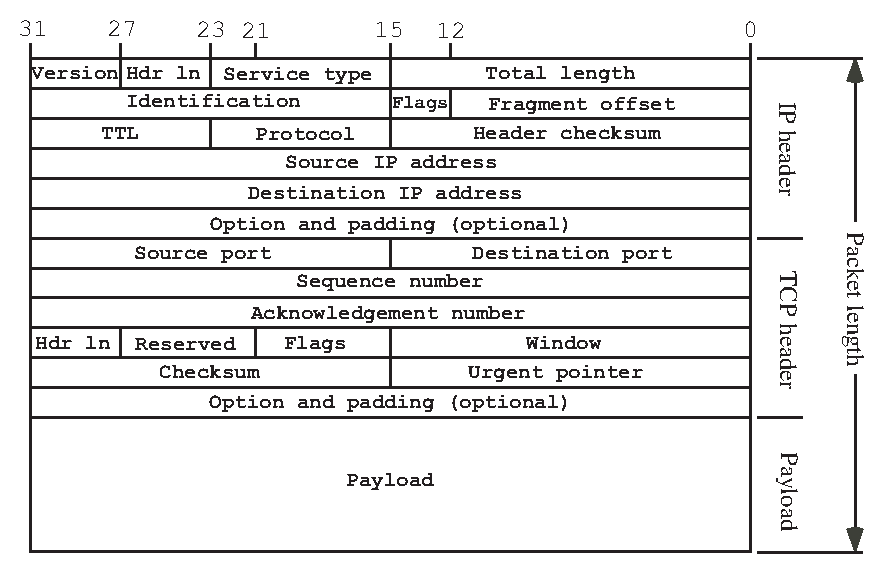
\includegraphics[width=0.9\textwidth]{source/fig/header.eps}}
    \caption[Structure of TCP/IP headers.]{Structure of TCP/IP headers used for host
    routing and byte stream reconstruction.}
    \label{c2:f1}
\end{figure}

\section{Motivations for Extended Research}\label{c2:s2}%
Whatever you can conclude...

Introduces next chapter if appropriate.
